%% abtex2-modelo-include-comandos.tex, v-1.9.6 laurocesar
%% Copyright 2012-2016 by abnTeX2 group at http://www.abntex.net.br/ 
%%
%% This work may be distributed and/or modified under the
%% conditions of the LaTeX Project Public License, either version 1.3
%% of this license or (at your option) any later version.
%% The latest version of this license is in
%%   http://www.latex-project.org/lppl.txt
%% and version 1.3 or later is part of all distributions of LaTeX
%% version 2005/12/01 or later.
%%
%% This work has the LPPL maintenance status `maintained'.
%% 
%% The Current Maintainer of this work is the abnTeX2 team, led
%% by Lauro César Araujo. Further information are available on 
%% http://www.abntex.net.br/
%%
%% This work consists of the files abntex2-modelo-include-comandos.tex
%% and abntex2-modelo-img-marca.pdf
%%

% ---
% Este capítulo, utilizado por diferentes exemplos do abnTeX2, ilustra o uso de
% comandos do abnTeX2 e de LaTeX.
% ---
 
\chapter{Referencial Teórico}\label{referecial_teorico}

% % escrever algo entre o inicio de cada capitulo 
% - Ultimo paragrafo da introdução , irei mencionar o abordado em cada capitulo 
% - Inicio de cada seção conter uma descrição 
% - Palavras em ingles italico \texitt
Neste capitulo é abordado o referencial teórico, utilizado como embasamento para a construção deste trabalho
% ---
\section{ Controle na Segurança Publica Brasileira }
Atualmente no Brasil existem dois sistemas informatizados utilizados por órgãos públicos para realizar a regulamentação e o monitoramento de armas de fogo, munições e demais produtos controlados.
Sendo estes,o Sistema de Gerenciamento Militar de Armas (SIGMA) e o Sistema Nacional de Armas (SINARM). O SIGMA é administrado pelo Exército Brasileiro e é responsável pelo controle de armas de fogo e munições no âmbito da Força. O SINARM é administrado pela Polícia Federal e é responsável pelo controle de armas de fogo e munições em poder da população civil.\cite{shotEntendaSinarm}

\subsection{SIGMA e SINARM}\label{sigmaesinarm}
A principal diferença entre SIGMA e SINARM é o âmbito de atuação. O SIGMA é responsável pelo controle de armas de fogo e munições no âmbito do Exército Brasileiro, enquanto o SINARM é responsável pelo controle de armas de fogo e munições em poder da população civil.
Outra diferença entre os dois sistemas é a natureza das informações que eles gerenciam. O SIGMA gerencia informações sobre armas de fogo e munições de uso militar, enquanto o SINARM gerencia informações sobre armas de fogo e munições de uso civil.
A seguir, está uma tabela comparativa que resume as principais diferenças entre ambos: 
\begin{table}[ht]
	\centering
	\caption{Comparação entre SIGMA e SINARM}
	\begin{tabularx}{\textwidth}{lXp{5cm}}
	  \toprule
	  Característica & SIGMA & SINARM \\
	  \midrule
	  Âmbito de atuação & Exército Brasileiro & População civil \\
	  Natureza das informações & Armas de fogo e munições de uso militar & Armas de fogo e munições de uso civil \\
	  Responsável pela administração & Exército Brasileiro & Polícia Federal \\
	  \bottomrule
	\end{tabularx}
  \end{table}

  
% \section{Segurança Publica - Integração SIGMA e SINARM}
% \cite[Em 2019, a Polícia Federal autorizou que o Exército tenha acesso ao Sinarm, já os militares não permitiram a liberação das informações do Sigma para os agentes da PF]{sbtnewsExxE9rcitoPolxEDcia}
% \cite{inDECRETO9847}

\section{ Sistema SIGMA } 
O Sistema de Gerenciamento Militar de Armas (SIGMA) é um sistema computacional desenvolvido pelo Centro de Desenvolvimento de Sistemas (CDS) do Exército Brasileiro e  implantado em 2003 que vem sendo constantemente atualizado para atender às necessidades da Força.\cite{fenemeReunixE3oSobre}

\subsection{Contexto de implantação}
O contexto da implantação do SIGMA foi a necessidade de modernizar o sistema de controle de armas de fogo e munições do Exército Brasileiro.
O SIGMA foi desenvolvido com base nas melhores práticas internacionais de controle de armas de fogo. O sistema é integrado a outros sistemas de informação do Exército Brasileiro, o que permite a troca de dados e informações entre as diferentes áreas da Força.\cite{fenemeReunixE3oSobre}

\subsection{AEL}
O Arquivo Eletrônico em Lote (AEL) é um arquivo digital que contém as informações necessárias para o cadastro produtos controlado no SIGMA.
O AEL é utilizado para o cadastro de armas de fogo de diversas entidades, como as Forças Armadas, as forças auxiliares, a Polícia Militar e o Corpo de Bombeiros.\cite{ExércitoBrasileiro}

O Objetivo do AEL no sistema SIGMA é permitir o cadastro de produtos controlados de diversas entidades de forma centralizada e organizada. O AEL é um elemento importante do SIGMA, pois permite que o Exército Brasileiro tenha um controle mais eficiente das armas de fogo em circulação no país\cite{ExércitoBrasileiro}

\subsection{Arquivo AEL na Brigada Militar do Rio Grande do Sul}
O AEL no contexto da BM RS, dever ser gerado para o cadastro de armas de fogo de policiais militares. O arquivo deve conter as seguintes informações:
\begin{itemize}
    \item Identificação da Brigada Militar: número do QG, código da OM e nome da OM.
    \item Identificação do armamento: número da arma, tipo de arma, marca, modelo, calibre, série.
    \item Identificação do proprietário: nome completo, CPF, RG, endereço e telefone.
\end{itemize}
Entre demais informações especificadas nos anexos \ref{sec:anexoA2} e \ref{sec:anexoA3}.

O AEL deve ser gerado em um formato texto, seguindo um layout pré-definido e estar conforme os parâmetros de indexação das informações constantes nos anexos \ref{sec:anexoA1} e \ref{sec:anexoA4}.

\section{Gerenciamento de processos}
É uma abordagem disciplinada e sistemática que envolve práticas relacionadas aos processos de negócio, automatizados ou não, com o objetivo de alcançar resultados consistentes e alinhados com as metas estratégicas de uma organização. 
Conforme\cite{davila2008inovaccao}''As organizações tentam inovar para se diferenciar e obter vantagens competitivas, tanto pela melhoria nos bens/serviços fornecidos quanto pela eficiência operativa''
Pode-se concluir que os sistemas de informação oferecem inúmeros benefícios para uma organização, sejam eles para melhorar o fluxo de informação, as tomadas decisões, controle de qualidade, ou ampliar a produtividade
\subsection{BPMN}
Modelo e notação de processos de negócios (\textit{Business Process Model and Notation}) é uma notação gráfica padronizada para desenhar processos de negócios em um fluxograma. A diagramação BPMN é intuitiva e permite a representação de detalhes complexos do processo. A simbologia deste modelo serve como uma linguagem padrão, colocando um fim na lacuna de comunicação entre a modelagem do processo e sua execução, para 
\begin{citacao}
	\cite{bitencourt2016elicitaccao} 
	Modelo de processos de negocio representa os processos de negocio de uma empresa e permite a documentação, simulação, compartilhamento, implementação, avaliação e melhoramento continuo das operações, com o intuito de compreender o funcionamento da organização e os aspectos do seu domínio
	
\end{citacao}
Em resumo, o levantamento e registro da situação atual dos processos, seguido por uma análise aprofundada, são práticas essenciais para promover a eficiência, a eficácia e a adaptação contínua dentro de uma organização. Essa abordagem sistemática para entender e aprimorar os processos é fundamental para a sustentabilidade organizacional.

\section{Padrões de Projeto de Sistemas}
Padrões de desenvolvimento de software referem-se a soluções reutilizáveis para problemas comuns encontrados no processo de desenvolvimento de software. Esses padrões são abstrações que encapsulam as melhores práticas, representando soluções testadas e comprovadas para desafios recorrentes. Eles fornecem diretrizes para o design e implementação de código, promovendo a consistência, a manutenibilidade e a eficiência no desenvolvimento de software.\cite{padroesProjeto}

O contexto dos padrões de desenvolvimento de software está relacionado aos desafios enfrentados pelos desenvolvedores ao criar sistemas de software complexos.Para \cite{padroesProjeto} ''Um padrão de projeto nomeia, abstrai e identifica aspectos problemáticos comuns e propõe uma solução padrão para esses problemas''


\subsection{Arquitetura Cliente Servidor}
Nessa arquitetura, o software é dividido em duas partes principais: o cliente e o servidor.
O cliente é a parte do sistema que interage diretamente com o usuário. Ele envia solicitações de serviço ao servidor e exibe os resultados recebidos ao usuário. O cliente pode ser um aplicativo de desktop, um aplicativo móvel ou um navegador da web, dependendo do tipo de sistema que está sendo desenvolvido.\cite{flanagan2012javascript}

O servidor é responsável por processar as solicitações recebidas do cliente e fornecer os recursos ou serviços solicitados. Ele possui os recursos necessários para atender às solicitações, como bancos de dados, aplicativos e serviços web. O servidor está sempre ativo, aguardando solicitações dos clientes e respondendo a elas de maneira apropriada.\cite{arqClientServer2}

A comunicação entre o cliente e o servidor ocorre por meio de uma rede, geralmente a Internet. O cliente envia uma solicitação para o servidor, especificando o tipo de serviço desejado e quaisquer parâmetros necessários.
Então de acordo com 
\begin{citacao}
	\cite{arqClientServer2} 
O servidor, quando recebe a mensagem, extrai os parâmetros 
e chama o procedimento especificado na mensagem. No fim da execução do procedimento é 
realizada a operação inversa, colocando os resultados e enviando a mensagem de resposta ao 
processo cliente
\end{citacao}

    Logo uma das principais vantagens da arquitetura cliente-servidor é a divisão clara de responsabilidades entre o cliente e o servidor. 
O cliente lida com a interface do usuário e a apresentação dos dados, enquanto o servidor cuida do processamento das solicitações e do acesso aos recursos. Isso permite uma melhor organização do sistema e facilita a manutenção e a escalabilidade.
Além disso, a arquitetura cliente-servidor permite que vários clientes acessem o mesmo servidor simultaneamente. Isso possibilita o compartilhamento de recursos e serviços, o que é especialmente útil em ambientes corporativos.\cite{arqClientServer2}

A \autoref{fig:grafico-client-server}demonstra a maneira como ocorre essa comunicação:

\begin{figure}[htb]
    \caption{\label{fig:grafico-client-server}Arquitetura Cliente-Servidor}
    \begin{center}
        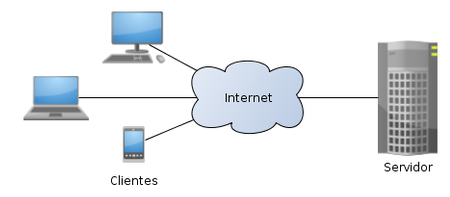
\includegraphics[scale=0.9]{imagens/arquitetura-cliente-servidor.png}
    \end{center}
    \legend{Fonte: \citeonline{RedesP2P67:online}}
\end{figure}


\subsection{Arquitetura MVC}
A arquitetura MVC \textit{Model-View-Controller} é um padrão de design que organiza o código de uma aplicação em três componentes principais: \textit{Model} (Modelo), \textit{View} (Visão) e \textit{Controller} (Controlador). Cada componente tem uma responsabilidade específica na aplicação, o que ajuda a manter o código modular, escalável e de fácil manutenção\cite{engsoftmoderna}

\begin{itemize}
    \item Visão: Lida com a apresentação dos dados ao usuário e interage com o Modelo. A Visão exibe as informações e envia eventos do usuário para o Controlador.
    \item Controlador: Recebe entradas do usuário, processa essas entradas (geralmente envolvendo o Modelo) e atualiza a Visão. O Controlador age como um intermediário entre o Modelo e a Visão.
    \item Modelo: Representa a lógica de negócios e os dados da aplicação. Geralmente, o modelo é responsável pela interação com o banco de dados e pela manipulação dos dados.
\end{itemize}
Conforme exemplificado o fluxo da arquitetura MVC na \autoref{fig:grafico-mvc}

\begin{figure}[htb]
    \caption{\label{fig:grafico-mvc}Arquitetura MVC}
    \begin{center}
        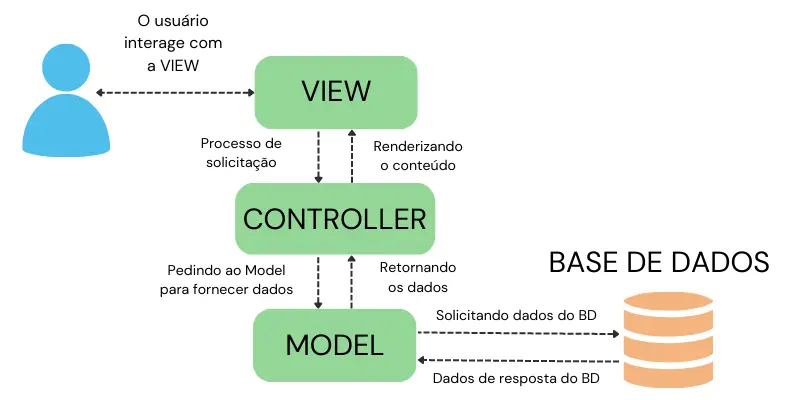
\includegraphics[scale=0.7]{imagens/arquitetura-mvc.png}
    \end{center}
    \legend{Fonte: \citeonline{engsoftmoderna}}
\end{figure}


\section{Aplicações Web}
Aplicações web são programas que são executados em navegadores e são acessados por meio de internet.
Surgiram na década de 1990 e se tornaram populares por permitirem a interação do usuário e o processamento de dados.

Existem dois tipos principais: estáticas (HTML, CSS e JavaScript) e dinâmicas (linguagens de programação do lado do servidor).
De acordo com\cite{aplicacoesWeb} as aplicações estáticas geralmente consistem em páginas web com conteúdo fixo, sem interação avançada ou processamento de dados em tempo real. O navegador do cliente solicita páginas estáticas ao servidor, que retorna arquivos HTML, CSS e JavaScript. A renderização e interação ocorrem no navegador.

Aplicações Dinâmicas apresentam interatividade avançada e processamento de dados em tempo real o navegador solicita uma página ao servidor. O servidor executa a lógica de negócios, acessa dados do banco de dados, gera dinamicamente o conteúdo HTML e o envia de volta ao navegador. Pode haver interações adicionais entre o navegador e o servidor \cite{aplicacoesWeb}
Conforme a \cite{amazonAplicaoWeb} oferecem diversos benefícios como acessibilidade, atualização, redução de custos e escalabilidade.

\subsection{Linguagem JavaScript}
Uma linguagem de programação amplamente usada no desenvolvimento web de acordo com a organização \cite{mozillaJavaScript}. Ela permite adicionar interatividade e dinamismo a páginas da web. Além de ser usado no desenvolvimento de interfaces de usuário, o JavaScript também pode ser usado no desenvolvimento de aplicativos do lado do servidor (backend) com o uso de tecnologias como o Node.js. Conforme \cite{flanagan2012javascript} ''Javascript já deixou para trás suas raízes como linguagem de script há muito tempo, tornando-se uma linguagem de uso geral, robusta e eficiente''

\subsection{Frameworks}
A necessidade da utilização de \textit{frameworks} surgiu com a complexidade crescente das aplicações de software.
Conforme abordado por: 
\begin{citacao}
	\cite{maldonado2002padroes} 
	Diversos \textit{frameworks} têm sido desenvolvidos nas duas últimas décadas, visando o
	reuso de software e consequentemente a melhoria da produtividade, qualidade e
	manutenibilidade
\end{citacao}
Sendo estes estruturas ou conjuntos de ferramentas que fornecem uma base organizada para o desenvolvimento de aplicações. Eles oferecem uma estrutura pré-definida que acelera o processo de desenvolvimento, promove a reutilização de código e estabelece padrões de boas práticas. No contexto do desenvolvimento de software, os frameworks desempenham um papel significativo, influenciando a forma como as aplicações são projetadas, implementadas e mantidas.\cite{maldonado2002padroes}

\subsubsection{Principais Frameworks Web}
Principais frameworks utilizados para o desenvolvimento de aplicações web 
\begin{itemize}\label{nodejs}
    \item Node: Conforme o site oficial do \cite{Nodejs}, ele é um ambiente de tempo de execução JavaScript que permite que o JavaScript seja executado no lado do servidor. Utilizando o mecanismo de JavaScript V8 do Google Chrome para executar código JavaScript fora do navegador.
	
    Com o Node.js, é possível criar aplicativos web e serviços \textit{backend} usando JavaScript. Ele fornece uma variedade de recursos e uma ampla gama de bibliotecas e frameworks, tornando-o uma escolha popular para o desenvolvimento de servidores e APIs. \cite{Nodejs}
    De acordo com 
    \begin{citacao}
        \cite{pereira2014aplicações} 
        Node.js é multiprotocolo, ou seja, com ele será possível trabalhar com os protocolos: HTTP, HTTPS, FTP, SSH, DNS, TCP, UDP, WebSockets e também existem outros.Toda aplicação web necessita de um servidor para disponibilizar todos os seus  recursos
    \end{citacao}

    \item Express: Framework para aplicativos web do lado do servidor construído em cima do framework abordado na \autoref{nodejs}. 
     Ele fornece uma abordagem simplificada para lidar com solicitações HTTP, roteamento e manipulação de middleware. 
	 O Express permite criar facilmente APIs robustas e eficientes, tornando o desenvolvimento de aplicativos web mais rápido e produtivo. É um dos frameworks mais populares para o desenvolvimento de servidores com Node.js 
     \cite{pereira2014aplicações}
    \item React: É uma biblioteca JavaScript \textit{Open Source} usada para criar interfaces de usuário. Ele permite criar componentes reutilizáveis e interativos para construir interfaces de usuário modernas e responsivas.  Tornando possível a criação de aplicações nativas com desempenho e controles nativos \cite{ReactMet54}.
    O React usa uma abordagem baseada em componentes, o que facilita a criação e o gerenciamento do estado dos elementos da interface.Permitindo a criação de aplicações eficientes e escaláveis.\cite{ReactMet54}
\end{itemize}

\section{Banco de dados NOSQL}
Banco de dados NoSQL é um tipo de banco de dados que difere dos bancos de dados relacionais tradicionais (SQL) em sua estrutura de armazenamento e modelo de dados. NoSQL significa \textit{Not Only SQL} (Não Apenas SQL) e abrange diversos tipos de bancos de dados que oferecem uma abordagem alternativa para o armazenamento e recuperação de dados.
conforme \cite{pereira2014aplicações} uma das vantagens em se trabalhar com um banco de dados desse modelo é o grande suporte oferecido pela comunidade do nodejs e uma vasta gama de compatibilidade com diversas tecnologias.
Dentre as principais tecnologias que tem uma alta sinergia nesse padrão não relacional são: 


\begin{itemize}
    \item MongoDB: um eficiente e popular de banco de dados NoSQL. Que utiliza um sistema de gerenciamento de banco de dados orientado a documentos, o que significa que os dados são armazenados em documentos semelhantes a JSON, em vez de tabelas com linhas e colunas como em um banco de dados relacional.\cite{pereira2014aplicações}
    Outra característica importante do MongoDB é sua capacidade de escalar horizontalmente. Oferecendo recursos avançados, como indexação, consultas poderosas e suporte a transações, tornando-o adequado para uma ampla gama de aplicações. É frequentemente utilizado em aplicativos web, análise de dados, e outras aplicações que exigem flexibilidade e escalabilidade \cite{pereira2014aplicações}
    \item Mongoose:  Uma biblioteca ODM \textit{Object Data Modeling} para Node.js e MongoDB. Sendo inserido como uma camada de abstração facilitando a conexão, modelagem de dados, a execução de consultas, e a interação com o banco de dados de maneira eficiente e organizada\cite{pereira2014aplicações}

\end{itemize}


% \section{Backend}
% É a parte de um sistema ou aplicação que lida com a lógica de negócios, processamento de dados e a comunicação com o banco de dados. Envolve a criação de servidores, APIs (Application Programming Interfaces) e serviços que fornecem os dados e funcionalidades necessárias para o funcionamento do sistema. Para o desenvolvimento backend, são utilizadas diversas tecnologias, como linguagens de programação (como JavaScript, Python, Java, etc.), bancos de dados (como MySQL, PostgreSQL, MongoDB, etc.) e frameworks (como Node.js, Django, Ruby on Rails, etc.). Então o backend deve ser capaz de servir ao front-end a comunicação em tempo real entre cliente e servidor — que seja rápido, atenda muitos usuários ao mesmo tempo e utilize recursos de I/O (dispositivos de entrada ou saída) de forma eficiente ( RIBEIRO, CAIO , 2013)

% \subsection{Apis Restful}

\subsection{Segurança e autenticação}
A segurança e autenticação em aplicações web são fundamentais para proteger dados e usuários. Utilizando criptografia,  e práticas de desenvolvimento seguro, é possível mitigar riscos, garantindo a integridade e confiabilidade do sistema. Estratégias como autenticação por token e hashing de senhas fortalecem a proteção, assegurando uma navegação online para o usuário segura e confiável.\cite{segurancaeauth}

\begin{itemize}
    \item Passport-Local: De acordo com o site oficial do \cite{passport84}, este é uma estratégia de autenticação fornecida pelo Passport.js para autenticar usuários usando um nome de usuário e senha em aplicativos Node.js. Ele é facilmente integrado a qualquer aplicativo ou framework que suporte middlewares do estilo \textit{Connect}, incluindo o Express. O Passport-local requer um retorno de chamada de verificação que valida as credenciais do usuário. Ele pode ser configurado para realizar a autenticação localmente, verificando o nome de usuário e a senha no banco de dados da aplicação. 
    \item Token JWT: \textit{JSON Web Token} (JWT) fornece uma abordagem segura para a troca de informações entre cliente e servidor por meio de um token gerado o qual o resultado final é um objeto JSON, conforme explicado por  
    \begin{citacao}
        \cite{segurancaeauth} 
        O token gerado pelo JWT é salvo
        no dispositivo do usuário e suas informações podem ser verificadas a cada solicitação,
        pois são criptografadas utilizando um segredo, através do algoritmo \textit{HMAC} ou de um par de chaves públicas e privadas, garantindo assim a sua confiabilidade
    \end{citacao}
    Na \autoref{fig:grafico-jwt} exemplifica o fluxo de autenticação por token jwt: 

\begin{figure}
    \caption{\label{fig:grafico-jwt} Fluxo de autenticação JWT}
    \begin{center}
        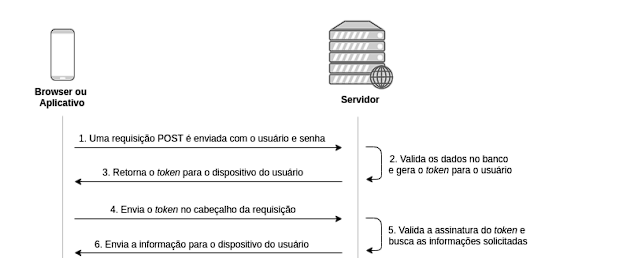
\includegraphics[scale=0.6]{imagens/jwt.png}
    \end{center}
    \legend{Fonte: \citeonline{segurancaeauth}}
\end{figure}
    
\end{itemize}

% \section{Frontend}
% É a parte de um sistema ou aplicação que os usuários interagem diretamente. Envolve a criação da interface do usuário, a implementação de elementos visuais, como layout, design, botões, formulários, etc., e a interação com o usuário por meio de eventos e ações. Para o desenvolvimento front-end, são utilizadas tecnologias como HTML (Hypertext Markup Language), CSS (Cascading Style Sheets) e JavaScript. Todo o HTML e o CSS que escrevemos ganha vida dentro dos navegadores utilizados por quem acessa nossas páginas e sites (MAZZA LUCAS, 2012)

% \begin{itemize}
%     \item HTML: (HyperText Markup Language) é a linguagem de marcação usada para estruturar e exibir o conteúdo de uma página da web. Ele fornece uma estrutura básica para a criação de elementos, como cabeçalhos, parágrafos, listas, links e imagens. O HTML é a espinha dorsal de qualquer página da web e é complementado por CSS e JavaScript para fornecer estilos e interatividade.
%     \item CSS: CSS (Cascading Style Sheets) é uma linguagem usada para estilizar a aparência dos elementos em uma página da web. Ele permite controlar cores, fontes, margens, posicionamento e outros aspectos visuais dos elementos HTML. O CSS é usado em conjunto com o HTML para criar layouts atraentes e responsivos. Ele oferece flexibilidade para personalizar o estilo de um site e torná-lo visualmente agradável para os usuários. 


% \end{itemize}
 





% ---

% A codificação de todos os arquivos do \abnTeX\ é \texttt{UTF8}. É necessário que
% você utilize a mesma codificação nos documentos que escrever, inclusive nos
% arquivos de base bibliográficas |.bib|.

% % ---
% \section{Citações diretas}
% \label{sec-citacao}
% % ---

% \index{citações!diretas}Utilize o ambiente \texttt{citacao} para incluir
% citações diretas com mais de três linhas:

% \begin{citacao}
% As citações diretas, no texto, com mais de três linhas, devem ser
% destacadas com recuo de 4 cm da margem esquerda, com letra menor que a do texto
% utilizado e sem as aspas. No caso de documentos datilografados, deve-se
% observar apenas o recuo \cite[5.3]{NBR10520:2002}.
% \end{citacao}

% Use o ambiente assim:

% \begin{verbatim}
% \begin{citacao}
% As citações diretas, no texto, com mais de três linhas [...] deve-se observar
% apenas o recuo \cite[5.3]{NBR10520:2002}.
% \end{citacao}
% \end{verbatim}

% O ambiente \texttt{citacao} pode receber como parâmetro opcional um nome de
% idioma previamente carregado nas opções da classe (\autoref{sec-hifenizacao}). Nesse
% caso, o texto da citação é automaticamente escrito em itálico e a hifenização é
% ajustada para o idioma selecionado na opção do ambiente. Por exemplo:

% \begin{verbatim}
% \begin{citacao}[english]
% Text in English language in italic with correct hyphenation.
% \end{citacao}
% \end{verbatim}

% Tem como resultado:

% \begin{citacao}[english]
% Text in English language in italic with correct hyphenation.
% \end{citacao}

% \index{citações!simples}Citações simples, com até três linhas, devem ser
% incluídas com aspas. Observe que em \LaTeX as aspas iniciais são diferentes das
% finais: ``Amor é fogo que arde sem se ver''.

% % ---
% \section{Notas de rodapé}
% % ---

% As notas de rodapé são detalhadas pela NBR 14724:2011 na seção 5.2.1\footnote{As
% notas devem ser digitadas ou datilografadas dentro das margens, ficando
% separadas do texto por um espaço simples de entre as linhas e por filete de 5
% cm, a partir da margem esquerda. Devem ser alinhadas, a partir da segunda linha
% da mesma nota, abaixo da primeira letra da primeira palavra, de forma a destacar
% o expoente, sem espaço entre elas e com fonte menor
% \citeonline[5.2.1]{NBR14724:2011}.}\footnote{Caso uma série de notas sejam
% criadas sequencialmente, o \abnTeX\ instrui o \LaTeX\ para que uma vírgula seja
% colocada após cada número do expoente que indica a nota de rodapé no corpo do
% texto.}\footnote{Verifique se os números do expoente possuem uma vírgula para
% dividi-los no corpo do texto.}. 




% % ---
% \section{Figuras}
% % ---

% \index{figuras}Figuras podem ser criadas diretamente em \LaTeX,
% como o exemplo da \autoref{fig_circulo}.

% \begin{figure}[htb]
% 	\caption{\label{fig_circulo}A delimitação do espaço}
% 	\begin{center}
% 	    \setlength{\unitlength}{5cm}
% 		\begin{picture}(1,1)
% 		\put(0,0){\line(0,1){1}}
% 		\put(0,0){\line(1,0){1}}
% 		\put(0,0){\line(1,1){1}}
% 		\put(0,0){\line(1,2){.5}}
% 		\put(0,0){\line(1,3){.3333}}
% 		\put(0,0){\line(1,4){.25}}
% 		\put(0,0){\line(1,5){.2}}
% 		\put(0,0){\line(1,6){.1667}}
% 		\put(0,0){\line(2,1){1}}
% 		\put(0,0){\line(2,3){.6667}}
% 		\put(0,0){\line(2,5){.4}}
% 		\put(0,0){\line(3,1){1}}
% 		\put(0,0){\line(3,2){1}}
% 		\put(0,0){\line(3,4){.75}}
% 		\put(0,0){\line(3,5){.6}}
% 		\put(0,0){\line(4,1){1}}
% 		\put(0,0){\line(4,3){1}}
% 		\put(0,0){\line(4,5){.8}}
% 		\put(0,0){\line(5,1){1}}
% 		\put(0,0){\line(5,2){1}}
% 		\put(0,0){\line(5,3){1}}
% 		\put(0,0){\line(5,4){1}}
% 		\put(0,0){\line(5,6){.8333}}
% 		\put(0,0){\line(6,1){1}}
% 		\put(0,0){\line(6,5){1}}
% 		\end{picture}
% 	\end{center}
% 	\legend{Fonte: os autores}
% \end{figure}

% Ou então figuras podem ser incorporadas de arquivos externos, como é o caso da
% \autoref{fig_grafico}. Se a figura que ser incluída se tratar de um diagrama, um
% gráfico ou uma ilustração que você mesmo produza, priorize o uso de imagens
% vetoriais no formato PDF. Com isso, o tamanho do arquivo final do trabalho será
% menor, e as imagens terão uma apresentação melhor, principalmente quando
% impressas, uma vez que imagens vetorias são perfeitamente escaláveis para
% qualquer dimensão. Nesse caso, se for utilizar o Microsoft Excel para produzir
% gráficos, ou o Microsoft Word para produzir ilustrações, exporte-os como PDF e
% os incorpore ao documento conforme o exemplo abaixo. No entanto, para manter a
% coerência no uso de software livre (já que você está usando \LaTeX e \abnTeX),
% teste a ferramenta \textsf{InkScape}\index{InkScape}
% (\url{http://inkscape.org/}). Ela é uma excelente opção de código-livre para
% produzir ilustrações vetoriais, similar ao CorelDraw\index{CorelDraw} ou ao Adobe
% Illustrator\index{Adobe Illustrator}. De todo modo, caso não seja possível
% utilizar arquivos de imagens como PDF, utilize qualquer outro formato, como
% JPEG, GIF, BMP, etc. Nesse caso, você pode tentar aprimorar as imagens
% incorporadas com o software livre \textsf{Gimp}\index{Gimp}
% (\url{http://www.gimp.org/}). Ele é uma alternativa livre ao Adobe
% Photoshop\index{Adobe Photoshop}.

% \begin{figure}[htb]
% 	\caption{\label{fig_grafico}Gráfico produzido em Excel e salvo como PDF}
% 	\begin{center}
% 	    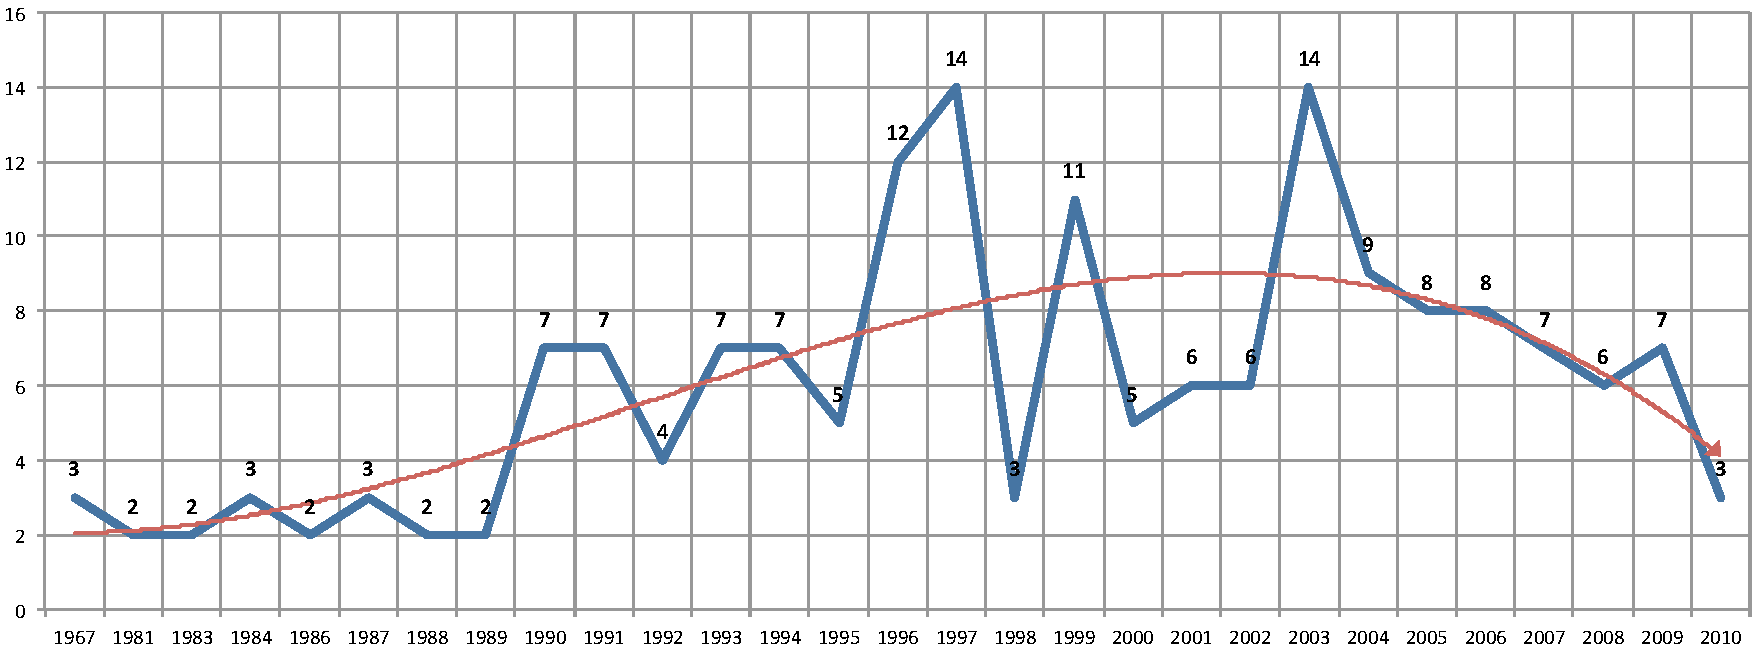
\includegraphics[scale=0.5]{imagens/abntex2-modelo-img-grafico.pdf}
% 	\end{center}
% 	\legend{Fonte: \citeonline[p. 24]{araujo2012}}
% \end{figure}

% % ---
% \subsection{Figuras em \emph{minipages}}
% % ---

% \emph{Minipages} são usadas para inserir textos ou outros elementos em quadros
% com tamanhos e posições controladas. Veja o exemplo da
% \autoref{fig_minipage_imagem1} e da \autoref{fig_minipage_grafico2}.

% \begin{figure}[htb]
%  \label{teste}
%  \centering
%   \begin{minipage}{0.4\textwidth}
%     \centering
%     \caption{Imagem 1 da minipage} \label{fig_minipage_imagem1}
%     
\includegraphics[scale=0.9]{imagens/abntex2-modelo-img-marca.pdf}
%     \legend{Fonte: Produzido pelos autores}
%   \end{minipage}
%   \hfill
%   \begin{minipage}{0.4\textwidth}
%     \centering
%     \caption{Grafico 2 da minipage} \label{fig_minipage_grafico2}
%     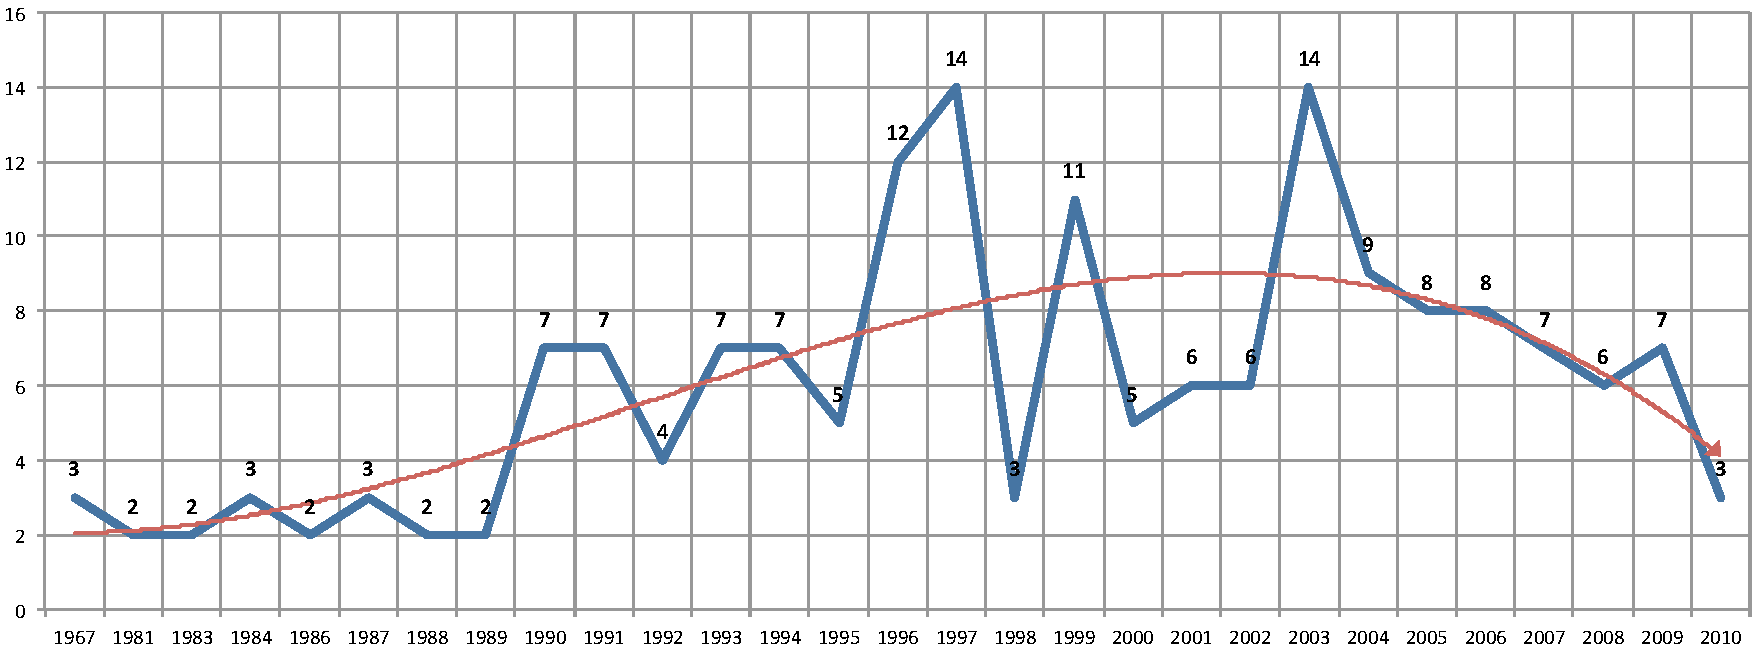
\includegraphics[scale=0.2]{imagens/abntex2-modelo-img-grafico.pdf}
%     \legend{Fonte: \citeonline[p. 24]{araujo2012}}
%   \end{minipage}
% \end{figure}

% Observe que, segundo a \citeonline[seções 4.2.1.10 e 5.8]{NBR14724:2011}, as
% ilustrações devem sempre ter numeração contínua e única em todo o documento:

% \begin{citacao}
% Qualquer que seja o tipo de ilustração, sua identificação aparece na parte
% superior, precedida da palavra designativa (desenho, esquema, fluxograma,
% fotografia, gráfico, mapa, organograma, planta, quadro, retrato, figura,
% imagem, entre outros), seguida de seu número de ordem de ocorrência no texto,
% em algarismos arábicos, travessão e do respectivo título. Após a ilustração, na
% parte inferior, indicar a fonte consultada (elemento obrigatório, mesmo que
% seja produção do próprio autor), legenda, notas e outras informações
% necessárias à sua compreensão (se houver). A ilustração deve ser citada no
% texto e inserida o mais próximo possível do trecho a que se
% refere. \cite[seções 5.8]{NBR14724:2011}
% \end{citacao}

% % ---
% \section{Expressões matemáticas}
% % ---

% \index{expressões matemáticas}Use o ambiente \texttt{equation} para escrever
% expressões matemáticas numeradas:

% \begin{equation}
%   \forall x \in X, \quad \exists \: y \leq \epsilon
% \end{equation}

% Escreva expressões matemáticas entre \$ e \$, como em $ \lim_{x \to \infty}
% \exp(-x) = 0 $, para que fiquem na mesma linha.

% Também é possível usar colchetes para indicar o início de uma expressão
% matemática que não é numerada.

% \[
% \left|\sum_{i=1}^n a_ib_i\right|
% \le
% \left(\sum_{i=1}^n a_i^2\right)^{1/2}
% \left(\sum_{i=1}^n b_i^2\right)^{1/2}
% \]

% Consulte mais informações sobre expressões matemáticas em
% \url{https://github.com/abntex/abntex2/wiki/Referencias}.

% % ---
% \section{Enumerações: alíneas e subalíneas}
% % ---

% \index{alíneas}\index{subalíneas}\index{incisos}Quando for necessário enumerar
% os diversos assuntos de uma seção que não possua título, esta deve ser
% subdividida em alíneas \cite[4.2]{NBR6024:2012}:

% \begin{alineas}

%   \item os diversos assuntos que não possuam título próprio, dentro de uma mesma
%   seção, devem ser subdivididos em alíneas; 
  
%   \item o texto que antecede as alíneas termina em dois pontos;
%   \item as alíneas devem ser indicadas alfabeticamente, em letra minúscula,
%   seguida de parêntese. Utilizam-se letras dobradas, quando esgotadas as
%   letras do alfabeto;

%   \item as letras indicativas das alíneas devem apresentar recuo em relação à
%   margem esquerda;

%   \item o texto da alínea deve começar por letra minúscula e terminar em
%   ponto-e-vírgula, exceto a última alínea que termina em ponto final;

%   \item o texto da alínea deve terminar em dois pontos, se houver subalínea;

%   \item a segunda e as seguintes linhas do texto da alínea começa sob a
%   primeira letra do texto da própria alínea;
  
%   \item subalíneas \cite[4.3]{NBR6024:2012} devem ser conforme as alíneas a
%   seguir:

%   \begin{alineas}
%      \item as subalíneas devem começar por travessão seguido de espaço;

%      \item as subalíneas devem apresentar recuo em relação à alínea;

%      \item o texto da subalínea deve começar por letra minúscula e terminar em
%      ponto-e-vírgula. A última subalínea deve terminar em ponto final, se não
%      houver alínea subsequente;

%      \item a segunda e as seguintes linhas do texto da subalínea começam sob a
%      primeira letra do texto da própria subalínea.
%   \end{alineas}
  
%   \item no \abnTeX\ estão disponíveis os ambientes \texttt{incisos} e
%   \texttt{subalineas}, que em suma são o mesmo que se criar outro nível de
%   \texttt{alineas}, como nos exemplos à seguir:
  
%   \begin{incisos}
%     \item \textit{Um novo inciso em itálico};
%   \end{incisos}
  
%   \item Alínea em \textbf{negrito}:
  
%   \begin{subalineas}
%     \item \textit{Uma subalínea em itálico};
%     \item \underline{\textit{Uma subalínea em itálico e sublinhado}}; 
%   \end{subalineas}
  
%   \item Última alínea com \emph{ênfase}.
  
% \end{alineas}

% % ---
% \section{Espaçamento entre parágrafos e linhas}
% % ---

% \index{espaçamento!dos parágrafos}O tamanho do parágrafo, espaço entre a margem
% e o início da frase do parágrafo, é definido por:

% \begin{verbatim}
%    \setlength{\parindent}{1.3cm}
% \end{verbatim}

% \index{espaçamento!do primeiro parágrafo}Por padrão, não há espaçamento no
% primeiro parágrafo de cada início de divisão do documento
% (\autoref{sec-divisoes}). Porém, você pode definir que o primeiro parágrafo
% também seja indentado, como é o caso deste documento. Para isso, apenas inclua o
% pacote \textsf{indentfirst} no preâmbulo do documento:

% \begin{verbatim}
%    \usepackage{indentfirst}      % Indenta o primeiro parágrafo de cada seção.
% \end{verbatim}

% \index{espaçamento!entre os parágrafos}O espaçamento entre um parágrafo e outro
% pode ser controlado por meio do comando:

% \begin{verbatim}
%   \setlength{\parskip}{0.2cm}  % tente também \onelineskip
% \end{verbatim}

% \index{espaçamento!entre as linhas}O controle do espaçamento entre linhas é
% definido por:

% \begin{verbatim}
%   \OnehalfSpacing       % espaçamento um e meio (padrão); 
%   \DoubleSpacing        % espaçamento duplo
%   \SingleSpacing        % espaçamento simples	
% \end{verbatim}

% Para isso, também estão disponíveis os ambientes:

% \begin{verbatim}
%   \begin{SingleSpace} ...\end{SingleSpace}
%   \begin{Spacing}{hfactori} ... \end{Spacing}
%   \begin{OnehalfSpace} ... \end{OnehalfSpace}
%   \begin{OnehalfSpace*} ... \end{OnehalfSpace*}
%   \begin{DoubleSpace} ... \end{DoubleSpace}
%   \begin{DoubleSpace*} ... \end{DoubleSpace*} 
% \end{verbatim}

% Para mais informações, consulte \citeonline[p. 47-52 e 135]{memoir}.

% % ---
% \section{Inclusão de outros arquivos}\label{sec-include}
% % ---

% É uma boa prática dividir o seu documento em diversos arquivos, e não
% apenas escrever tudo em um único. Esse recurso foi utilizado neste
% documento. Para incluir diferentes arquivos em um arquivo principal,
% de modo que cada arquivo incluído fique em uma página diferente, utilize o
% comando:

% \begin{verbatim}
%    \include{documento-a-ser-incluido}      % sem a extensão .tex
% \end{verbatim}

% Para incluir documentos sem quebra de páginas, utilize:

% \begin{verbatim}
%    \input{documento-a-ser-incluido}      % sem a extensão .tex
% \end{verbatim}

% % ---
% \section{Compilar o documento \LaTeX}
% % ---

% Geralmente os editores \LaTeX, como o
% TeXlipse\footnote{\url{http://texlipse.sourceforge.net/}}, o
% Texmaker\footnote{\url{http://www.xm1math.net/texmaker/}}, entre outros,
% compilam os documentos automaticamente, de modo que você não precisa se
% preocupar com isso.

% No entanto, você pode compilar os documentos \LaTeX usando os seguintes
% comandos, que devem ser digitados no \emph{Prompt de Comandos} do Windows ou no
% \emph{Terminal} do Mac ou do Linux:

% \begin{verbatim}
%    pdflatex ARQUIVO_PRINCIPAL.tex
%    bibtex ARQUIVO_PRINCIPAL.aux
%    makeindex ARQUIVO_PRINCIPAL.idx 
%    makeindex ARQUIVO_PRINCIPAL.nlo -s nomencl.ist -o ARQUIVO_PRINCIPAL.nls
%    pdflatex ARQUIVO_PRINCIPAL.tex
%    pdflatex ARQUIVO_PRINCIPAL.tex
% \end{verbatim}

% % ---
% \section{Remissões internas}
% % ---

% Ao nomear a \autoref{tab-nivinv} e a \autoref{fig_circulo}, apresentamos um
% exemplo de remissão interna, que também pode ser feita quando indicamos o
% \autoref{cap_exemplos}, que tem o nome \emph{\nameref{cap_exemplos}}. O número
% do capítulo indicado é \ref{cap_exemplos}, que se inicia à
% \autopageref{cap_exemplos}\footnote{O número da página de uma remissão pode ser
% obtida também assim:
% \pageref{cap_exemplos}.}.
% Veja a \autoref{sec-divisoes} para outros exemplos de remissões internas entre
% seções, subseções e subsubseções.

% O código usado para produzir o texto desta seção é:

% \begin{verbatim}
% Ao nomear a \autoref{tab-nivinv} e a \autoref{fig_circulo}, apresentamos um
% exemplo de remissão interna, que também pode ser feita quando indicamos o
% \autoref{cap_exemplos}, que tem o nome \emph{\nameref{cap_exemplos}}. O número
% do capítulo indicado é \ref{cap_exemplos}, que se inicia à
% \autopageref{cap_exemplos}\footnote{O número da página de uma remissão pode ser
% obtida também assim:
% \pageref{cap_exemplos}.}.
% Veja a \autoref{sec-divisoes} para outros exemplos de remissões internas entre
% seções, subseções e subsubseções.
% \end{verbatim}

% % ---
% \section{Divisões do documento: seção}\label{sec-divisoes}
% % ---

% Esta seção testa o uso de divisões de documentos. Esta é a
% \autoref{sec-divisoes}. Veja a \autoref{sec-divisoes-subsection}.

% \subsection{Divisões do documento: subseção}\label{sec-divisoes-subsection}

% Isto é uma subseção. Veja a \autoref{sec-divisoes-subsubsection}, que é uma
% \texttt{subsubsection} do \LaTeX, mas é impressa chamada de ``subseção'' porque
% no Português não temos a palavra ``subsubseção''.

% \subsubsection{Divisões do documento: subsubseção}
% \label{sec-divisoes-subsubsection}

% Isto é uma subsubseção.

% \subsubsection{Divisões do documento: subsubseção}

% Isto é outra subsubseção.

% \subsection{Divisões do documento: subseção}\label{sec-exemplo-subsec}

% Isto é uma subseção.

% \subsubsection{Divisões do documento: subsubseção}

% Isto é mais uma subsubseção da \autoref{sec-exemplo-subsec}.


% \subsubsubsection{Esta é uma subseção de quinto
% nível}\label{sec-exemplo-subsubsubsection}

% Esta é uma seção de quinto nível. Ela é produzida com o seguinte comando:

% \begin{verbatim}
% \subsubsubsection{Esta é uma subseção de quinto
% nível}\label{sec-exemplo-subsubsubsection}
% \end{verbatim}

% \subsubsubsection{Esta é outra subseção de quinto nível}\label{sec-exemplo-subsubsubsection-outro}

% Esta é outra seção de quinto nível.


% \paragraph{Este é um parágrafo numerado}\label{sec-exemplo-paragrafo}

% Este é um exemplo de parágrafo nomeado. Ele é produzida com o comando de
% parágrafo:

% \begin{verbatim}
% \paragraph{Este é um parágrafo nomeado}\label{sec-exemplo-paragrafo}
% \end{verbatim}

% A numeração entre parágrafos numeradaos e subsubsubseções são contínuas.

% \paragraph{Esta é outro parágrafo numerado}\label{sec-exemplo-paragrafo-outro}

% Esta é outro parágrafo nomeado.

% % ---
% \section{Este é um exemplo de nome de seção longo. Ele deve estar
% alinhado à esquerda e a segunda e demais linhas devem iniciar logo abaixo da
% primeira palavra da primeira linha}
% % ---

% Isso atende à norma \citeonline[seções de 5.2.2 a 5.2.4]{NBR14724:2011} 
%  e \citeonline[seções de 3.1 a 3.8]{NBR6024:2012}.

% % ---
% \section{Diferentes idiomas e hifenizações}
% \label{sec-hifenizacao}
% % ---

% Para usar hifenizações de diferentes idiomas, inclua nas opções do documento o
% nome dos idiomas que o seu texto contém. Por exemplo (para melhor
% visualização, as opções foram quebras em diferentes linhas):

% \begin{verbatim}
% \documentclass[
% 	12pt,
% 	openright,
% 	twoside,
% 	a4paper,
% 	english,
% 	french,
% 	spanish,
% 	brazil
% 	]{abntex2}
% \end{verbatim}

% O idioma português-brasileiro (\texttt{brazil}) é incluído automaticamente pela
% classe \textsf{abntex2}. Porém, mesmo assim a opção \texttt{brazil} deve ser
% informada como a última opção da classe para que todos os pacotes reconheçam o
% idioma. Vale ressaltar que a última opção de idioma é a utilizada por padrão no
% documento. Desse modo, caso deseje escrever um texto em inglês que tenha
% citações em português e em francês, você deveria usar o preâmbulo como abaixo:

% \begin{verbatim}
% \documentclass[
% 	12pt,
% 	openright,
% 	twoside,
% 	a4paper,
% 	french,
% 	brazil,
% 	english
% 	]{abntex2}
% \end{verbatim}

% A lista completa de idiomas suportados, bem como outras opções de hifenização,
% estão disponíveis em \citeonline[p.~5-6]{babel}.

% Exemplo de hifenização em inglês\footnote{Extraído de:
% \url{http://en.wikibooks.org/wiki/LaTeX/Internationalization}}:

% \begin{otherlanguage*}{english}
% \textit{Text in English language. This environment switches all language-related
% definitions, like the language specific names for figures, tables etc. to the other
% language. The starred version of this environment typesets the main text
% according to the rules of the other language, but keeps the language specific
% string for ancillary things like figures, in the main language of the document.
% The environment hyphenrules switches only the hyphenation patterns used; it can
% also be used to disallow hyphenation by using the language name
% `nohyphenation'.}
% \end{otherlanguage*}

% Exemplo de hifenização em francês\footnote{Extraído de:
% \url{http://bigbrowser.blog.lemonde.fr/2013/02/17/tu-ne-tweeteras-point-le-vatican-interdit-aux-cardinaux-de-tweeter-pendant-le-conclave/}}:

% \begin{otherlanguage*}{french}
% \textit{Texte en français. Pas question que Twitter ne vienne faire une
% concurrence déloyale à la traditionnelle fumée blanche qui marque l'élection
% d'un nouveau pape. Pour éviter toute fuite précoce, le Vatican a donc pris un
% peu d'avance, et a déjà interdit aux cardinaux qui prendront part au vote
% d'utiliser le réseau social, selon Catholic News Service. Une mesure valable
% surtout pour les neuf cardinaux – sur les 117 du conclave – pratiquants très
% actifs de Twitter, qui auront interdiction pendant toute la période de se
% connecter à leur compte.}
% \end{otherlanguage*}

% Pequeno texto em espanhol\footnote{Extraído de:
% \url{http://internacional.elpais.com/internacional/2013/02/17/actualidad/1361102009_913423.html}}:

% \foreignlanguage{spanish}{\textit{Decenas de miles de personas ovacionan al pontífice en su
% penúltimo ángelus dominical, el primero desde que anunciase su renuncia. El Papa se
% centra en la crítica al materialismo}}.

% O idioma geral do texto por ser alterado como no exemplo seguinte:

% \begin{verbatim}
%   \selectlanguage{english}
% \end{verbatim}

% Isso altera automaticamente a hifenização e todos os nomes constantes de
% referências do documento para o idioma inglês. Consulte o manual da classe
% \cite{abntex2classe} para obter orientações adicionais sobre internacionalização de
% documentos produzidos com \abnTeX.

% A \autoref{sec-citacao} descreve o ambiente \texttt{citacao} que pode receber
% como parâmetro um idioma a ser usado na citação.

% % ---
% \section{Consulte o manual da classe \textsf{abntex2}}
% % ---

% Consulte o manual da classe \textsf{abntex2} \cite{abntex2classe} para uma
% referência completa das macros e ambientes disponíveis. 

% Além disso, o manual possui informações adicionais sobre as normas ABNT
% observadas pelo \abnTeX\ e considerações sobre eventuais requisitos específicos
% não atendidos, como o caso da \citeonline[seção 5.2.2]{NBR14724:2011}, que
% especifica o espaçamento entre os capítulos e o início do texto, regra
% propositalmente não atendida pelo presente modelo.

% % ---
% \section{Referências bibliográficas}
% % ---

% A formatação das referências bibliográficas conforme as regras da ABNT são um
% dos principais objetivos do \abnTeX. Consulte os manuais
% \citeonline{abntex2cite} e \citeonline{abntex2cite-alf} para obter informações
% sobre como utilizar as referências bibliográficas.

% %-
% \subsection{Acentuação de referências bibliográficas}
% %-

% Normalmente não há problemas em usar caracteres acentuados em arquivos
% bibliográficos (\texttt{*.bib}). Porém, como as regras da ABNT fazem uso quase
% abusivo da conversão para letras maiúsculas, é preciso observar o modo como se
% escreve os nomes dos autores. Na ~\autoref{tabela-acentos} você encontra alguns
% exemplos das conversões mais importantes. Preste atenção especial para `ç' e `í'
% que devem estar envoltos em chaves. A regra geral é sempre usar a acentuação
% neste modo quando houver conversão para letras maiúsculas.

% % ---
% \section{Precisa de ajuda?}
% % ---

% Consulte a FAQ com perguntas frequentes e comuns no portal do \abnTeX:
% \url{https://github.com/abntex/abntex2/wiki/FAQ}.

% Inscreva-se no grupo de usuários \LaTeX:
% \url{http://groups.google.com/group/latex-br}, tire suas dúvidas e ajude
% outros usuários.

% Participe também do grupo de desenvolvedores do \abnTeX:
% \url{http://groups.google.com/group/abntex2} e faça sua contribuição à
% ferramenta.

% % ---
% \section{Você pode ajudar?}
% % ---

% Sua contribuição é muito importante! Você pode ajudar na divulgação, no
% desenvolvimento e de várias outras formas. Veja como contribuir com o \abnTeX\
% em \url{https://github.com/abntex/abntex2/wiki/Como-Contribuir}.

% % ---
% \section{Quer customizar os modelos do \abnTeX\ para sua instituição ou
% universidade?}
% % ---

% Veja como customizar o \abnTeX\ em:
% \url{https://github.com/abntex/abntex2/wiki/ComoCustomizar}.

